\section{The shell}

\begin{frame}{What is a shell?}

\begin{block}{Shell}
Simply put, the shell is a program that takes commands from the keyboard and gives them to the operating system to perform\cite{whatIsTheShell}.
\end{block}

\begin{figure}
	\centering
	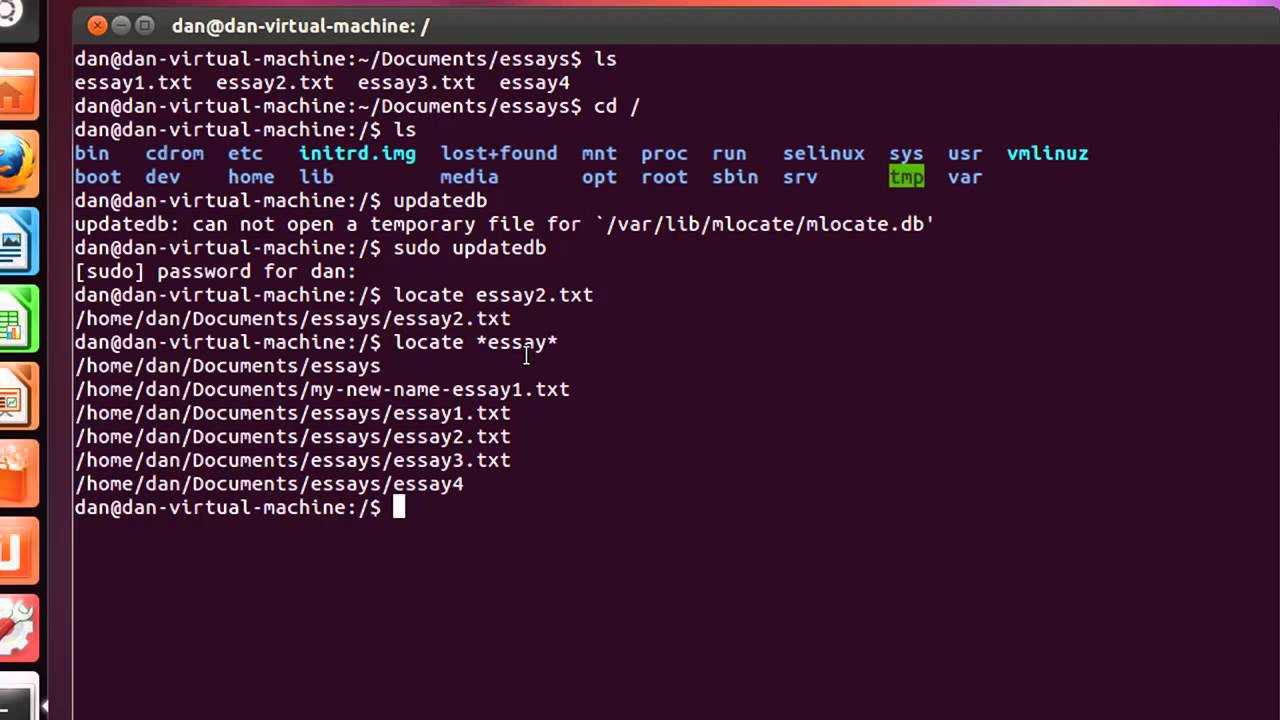
\includegraphics[width=1.0\textwidth]{terminal}
\end{figure}

\end{frame}

\begin{frame}{Shells implementations}
	A shell is an abstract concept. There are several implementations of a \code{shell}. Linux has different shells like \textit{bash}, \textit{sh}, \textit{ksh}. As for Windows, it has \textit{cmd} and \textit{power shell}.
	
	Each shell uses a different syntax for give commands ot the operating system. For instance:
	\begin{itemize}
		\item linux uses \code{ls -l} to print the files within a directory;
		\item windows uses \code{dir} to print the files within a directory;
	\end{itemize}
	
	Shells' syntaxes are theoretically different, but in reality they share lots fo similarities.
	
	\begin{note}
		We will show you \code{bash}, one of the most popular shells in linux.
	\end{note}
\end{frame}

\subsection{Base concepts}

\begin{frame}{Open the shell}
	The shell has different names depending on your operating system. For example:
	\begin{itemize}
		\item Ubuntu: click on Unity bar (top icon on the left side) and type \mdQuote{terminal}. Click the icon to start the terminal \cite{ubuntu:openterminal};
		\item Gnome: \mdQuote{gnome-terminal};
		\item lxUbuntu: \mdQuote{lxterminal};
	\end{itemize}
	
	The shell will start in some directory in your system. For example is may start in \code{/home/your-username/};
\end{frame}

\begin{frame}{Command structure}
	Each command in \code{bash} has the following structure\cite{command:structure}:
	
	\begin{parcenter}[1pt]
		\texttt{command-name command-options command-arguments}
	\end{parcenter}	
	
	For example:
	
	\begin{parcenter}[1pt]
		\code{mkdir -p -v --mode=777 "hello/world"}
	\end{parcenter}
	
	\only<1>{
	\begin{enumerate}
		\item \code{command-name} is the name of the command, in this case \mdQuote{mkdir};
		\item \code{command options} area is an optional part of the command. It represents some flags, options that slightly alter the command behaviour. For example here the options are \mdQuote{-pv --mode=777}.
		\item \code{command arguments} (if any) represents the value the command mainly operate with. They are not prefixed by any \mdQuote{-} character whatsoever. For example \mdQuote{"hello/world"} represents the command arguments.
	\end{enumerate}
	}
	
	\only<2>{
		Options can be typed using 2 conventions: 
		\begin{itemize}
			\item \textbf{brief}(\code{-p}): Typically (but not always) \textit{brief} options have 1 \mdQuote{-} and one character. For example the command has 2 brief options, \code{-p} and \code{-v}. Brief options can be merged: for example typing \mdQuote{-p -v} is always equal (except in few instances) to \mdQuote{-pv}. 
			\item \textbf{long}(\code{--mode}): They are typically (but not always) prefixed by \mdQuote{--}. They are usually composed by more than one character (\ie \mdQuote{mode}).
		\end{itemize}
	}
	
	\only<3>{
		Both \textit{brief} and \textit{long} options can accept arguments. Normally it done using this syntax:
		\begin{itemize}
			\item \textbf{brief}: in general you type the character representing the option, a space and the value of the option (\ie{} \code{-m 777});
			\item \textbf{long}: in general you type the string of the option, a \mdQuote{=} and th value of the option(\ie{} \code{--mode=777});
		\end{itemize}
		
		\begin{note}
			Most options in most commands have both a \textit{brief} and a \textit{long} name. For instance, \mdQuote{-m} and \mdQuote{--mode} for \code{mkdir} commands are synonyms.
		\end{note}
	}
		
\end{frame}

\begin{frame}{Return value}
	Each command has a \textbf{return value}, which is an integer. If the return value of a command is 0, everything was successful; otherwise an error occured while executing the command. You can get the return value of the last command executed with \code{\textdollar{}?}.
	
	
\end{frame}

\subsection{Commands}

\begin{frame}{Really basic command}

	\only<1>{
		\begin{block}{man}
			\code{man} stands for \textbf{MANual}. If you want to know all the details about a command, invoke its manual. For example, if you want to know the details of \code{ls}, type \code{man ls}. Basically you type \code{man} followed by a space followed by the name of the command you want to read about. If you don't know the exact syntax of a command, be super sure to check its manual before asking questions! If people, after listening to a question of yours, reply with \mdQuote{RTFM}, it means you should have read the manual (RTFM stands for \mdQuote{\textbf{R}ead \textbf{T}he \textbf{F}unny/\textbf{F}*****g \textbf{M}anual}).
		\end{block}
	}
	
	\only<2>{
		The man contains lots fo useful information: the available options of a command, how to use it, scenarios where it can be successfully used and how to interpret possibly errors.
		
		\begin{note}
			If you want some examples for a particular command, the MAN may have them as well.
		\end{note}
	}
	
	\only<3>{
		If \code{man} doesn't help you out, you may try \code{info command-name}. This is an explorable manual containing more information about the command. You may find additional examples here too.
		
		If you can't still find an example, try go to google and type \mdQuote{command\_you\_want examples}: for instance, you may google \mdQuote{grep examples} or \mdQuote{grep tutorial}.
	}
	
	\only<4>{
		\begin{block}{echo}
			Prints a string on the console. For example \code{echo "Hello world!"}
		\end{block}
	}
	
\end{frame}

\begin{frame}{Exercise}

	\begin{enumerate}
		\item<1-> What \code{mkdir} command does?
		\item<2-> Tell me an example of command option (both brief and long) of command \code{mkdir};
		\item<3-> How many arguments it can accept?
	\end{enumerate}
	
\end{frame}

\begin{frame}{File system exploration}

	\begin{block}{pwd}
		\code{pwd} will return the \textbf{absolute path} of the directory you're currently in. Super useful if you got lost in the file system.
	\end{block}
	
	\begin{block}{ls}
		returns the list of files (and directories) in the directory you're in. The options of this command tweak the information and the order used to output the content of a directory
	\end{block}
	
	\begin{block}{cd}
		Enters in a subdirectory inside \code{pwd}. Every directory has the directory \code{..}, representing the parent of the directory itself, and the directory \code{.}, representing the directory itself. Hence, the direcotry \mdQuote{/home/koldar/} has a subdirectory called \code{..} pointing to \code{/home/} and a directory called \code{.}, pointing to \code{/home/koldar/}.
	\end{block}

\end{frame}

\begin{frame}{Exercises}
	\begin{enumerate}
		\item<1-> list of the files in a directory (even the \textit{hidden ones}, namely the files starting with \mdQuote{.});
		\item<2-> list the content of the directory by size: the first one is the biggest file while the last in the list is the smallest one;
		\item<3-> retrieve the version of the command \mdQuote{pwd};
	\end{enumerate}
\end{frame}

\begin{frame}{File system manipulation}

	\begin{block}{mkdir}
		Creates a directory in the current working directory.
	\end{block}
	
	\begin{block}{rmdir}
		Remove an empty directory from the file system.
	\end{block}
	
	\begin{block}{rm}
		Remove one or more directories from the file system.
	\end{block}
	
	\begin{block}{touch}
		update to the current time the \mdQuote{last modified date} of a file. Creates the file if it doesn't exist.
	\end{block}
	
	\begin{block}{nano}
		Open a (simplicistic) editor used to alter files. Use \keystroke{Ctrl} + \keystroke{X} to save and exit.
	\end{block}

\end{frame}

\begin{frame}{Exercise}

	\begin{enumerate}
		\item<1-> Create a directory called \mdQuote{hello}?
		\item<2-> Inside it, create a file \mdQuote{world}.
		\item<3-> Inside file \mdQuote{world}, write \mdQuote{hello world};
		\item<4-> save and exit the file.
		\item<3-> Create a copy of \mdQuote{world} file, called \mdQuote{world2}. Use \code{cp} command.
	\end{enumerate}
	
\end{frame}

\begin{frame}{File manipulation}
	\only<1>{
		\begin{block}{cp}
			Copy files and directories. For example \code{cp file\_to\_copy name\_of\_copy}
		\end{block}
		
		\begin{block}{mv}
			Cut files and directory and paste them in another place. You can use this command to rename files as well (\eg \code{mv hello world}).
		\end{block}
		
		\begin{block}{cat}
			Concatenate several files content in a single output. You can use it to view the content of a single file as well (\eg \code{cat hello}).
		\end{block}
	}
	
	\only<2>{
		\begin{block}{less}
			Read a file. This is an awesome reader which can even several useful commands. You can view the commands in \code{less} by pressing \mdQuote{h} when less is executing.
		\end{block}
		
		\begin{block}{tail}
			Prints the last $n$ lines of a file.
		\end{block}
		
		\begin{block}{head}
			Prints the first $n$ lines of a file.
		\end{block}
	}
\end{frame}

\begin{frame}{Miscellanea}
	\begin{block}{history}
		Allows you to view the last commands you've put in the bash. Useful if you don't remember a command you've executed.
	\end{block}
	
	\begin{block}{wget}
		Download a file from the internet.
	\end{block}
	
	\begin{block}{grep}
		Given a list of text lines, retrieve only the ones containing a particular pattern. The most common use is \code{cat "DivinaCommedia" | grep "Virgilio"} (at the moment ignore the character \code{|}).
	\end{block}
\end{frame}

\begin{frame}{Exercise}
	\begin{enumerate}
		\item<1-> download the html page \code{https://en.wikipedia.org/wiki/Artificial\_intelligence}
		\item<2-> save the just downloaded page with \mdQuote{AI.html}
		\item<3-> use less to view the HTML code of the page;
		\item<4-> What is the character set of the page? (Hint: search \mdQuote{charset} in the top of the page);
		\item<5-> Search every link of JPG file in the downloaded page (Hint: use \code{grep} as explained before by matching the PDF extension: every JPG has it!);
		\item<6-> Download a JPG you want and look at the awesomeness that is artificial intelligence!
	\end{enumerate}
\end{frame}

\subsection{Advanced topics}

\begin{frame}{Wildcard}

Most commands accept wildcards in their filename or strings. A \textbf{wildcard} is a character (\textbf{*}) that means  \textit{whatever string, I don't care}. A classic example is \code{rm} command. Assume you have a directory filled with log files (text files with extension \mdQuote{.log}). You may remove one file per time with \code{rm}; or you can type:

\begin{center}
	\code{rm *.log}
\end{center}

The command stands for \textit{Removes everything in the current working directory that has whatever name but ends with \mdQuote{.log}}. Basically removes all the logs files.

Another great example is grep:

\begin{center}
	\code{ls -l | grep *.log}
\end{center}

It consider only the files and directories which end with \mdQuote{.log}.

\end{frame}

\begin{frame}[fragile]{Pipeline}
	\only<1->
	\begin{block}{Pipeline}
		Given the syntax \code{command-x command-options-x command-arguments-x | command-y command-options-y command-arguments-y} the pipeline allows to pass the standard output of command \code{command-x} as standard input of command \code{command-y}.
	\end{block}
\end{frame}

\begin{frame}[fragile]{Example of pipeline}

	For example, \code{ls -l  | grep "tex"} pass the standard output of the command \code{ls -l}, naley something like:
\begin{verbatim}
total 24
drwxrwxr-x 2 koldar koldar 4096 feb  6 14:21 build
-rw-rw-r-- 1 koldar koldar 1555 feb  5 15:46 main.tex
-rw-rw-r-- 1 koldar koldar  920 gen 17 14:47 Makefile
-rw-rw-r-- 1 koldar koldar 2053 feb  5 11:28 phd.sty
-rw-rw-r-- 1 koldar koldar 1172 feb  5 23:09 session.tks
drwxrwxr-x 7 koldar koldar 4096 feb  5 11:49 src
\end{verbatim}
	to the command \code{grep "tex"}. Since tex occurs only in the third line, the output of \code{ls -l  | grep "tex"} is:
\begin{verbatim}
-rw-rw-r-- 1 koldar koldar 1555 feb  5 15:46 main.tex
\end{verbatim}
\end{frame}

\begin{frame}{Bash Scripts}
	Instead of typing the same commands over and over, you can create a script containing for each line a command.
	When executing the script, the operating system will execute the commands contained in the script.
	
	\begin{block}{Script}
		A Bash script is a plain text file which contains a series of commands.\cite{bash:script}
	\end{block}
\end{frame}

\begin{frame}[fragile]{Simplest bash script ever!}
\begin{verbatim}
#!/bin/bash
# A sample Bash script, by Ryan
echo "Hello World!"
\end{verbatim}

Call the script\cite{bash:script} something like "mario.bash" and run the command \code{chmod u+x mario.bash}.
To execute it, type \code{./mario.bash}.

\begin{note}
Comments in bash scripts starts with \mdQuote{\#}. The first comment in the script above is \textbf{mandatory}.
Everything you put in bash scripts can be manually typed on the shell terminal as well.
\end{note}
\end{frame}

\begin{frame}[fragile]{Variables}
	You can define variables in scripts as well. Generally to create a variable (notice the \textbf{absence} of spaces):
	
\begin{verbatim}
VARIABLE_NAME=VARIABLE_VALUE
\end{verbatim}

	To use the variable value you can use:
	
\begin{verbatim}
${VARIABLE_NAME}
\end{verbatim}

	Variables are replaced inside \code{"} as well! Here a full example:
	
\begin{verbbox}
	#!/bin/bash
	echo "Enter your name:"
	read your_name
	echo "Your name is \textdollar{your_name}"
\end{verbbox}
\fbox{\theverbbox[t]}

\end{frame}